\chapter{Basic Statistics} \label{ch:statisticsandsampling}

Statistics is widely used in science and engineering. Broadly speaking, any attempt to estimate an unknown property of a system using direct or indirect measurements can be considered an application of statistics. Due to factors such as measurement errors and limited sample sizes, the exact value of the unknown property cannot be determined. Instead, statistics provides methodologies for efficiently estimating the most probable value of the unknown, given the available data and its limitations. It also offers tools to quantify the estimation error and the confidence level of the result.

This chapter introduces various sampling methods and demonstrates how to use samples to solve basic statistical problems.

\section{Two Types of Statistical Problems}

At least two common types of problems in science and engineering involve the widespread use of statistics.

\begin{enumerate}
	\item There is a property of the system whose true value exists but is unknown. We have either direct or indirect measurements of this value, subject to measurement noise. The goal is to estimate the true value from the measurements, while minimizing the effect of noise.

Example: Consider a power system with many buses, each having a voltage phasor. The objective is to estimate the voltage phasors using various sensor measurements deployed across the system.

	\item There is a large population of items whose properties follow an unknown underlying distribution. It is impractical to examine every item due to the size of the population. Hence, we collect some samples and record their properties. The goal is to estimate the distribution of the entire population using only the samples.

Example: Suppose a factory produces a large number of light bulbs. The objective is to estimate the average lifespan of the bulbs by randomly selecting a few and testing their durability.

\end{enumerate}

The two types of problems, though sound different, are deeply connected in the essence. Specifically, the first type will be introduced with greater details in control system relevant notebooks.

\section{Sampling}

When selecting samples from the population, it is critical to ensure that the selection is done randomly, and all elements in the population have an equal probability of being selected. 

Depending on whether an element can be selected multiple times, we have
\begin{itemize}
  \item Sampling with replacement. In this scenario, a member can be chosen more than once, and the samples are \mync{independent and identically distributed}[i.i.d.]
  \item Sampling without replacement. In this scenario, a member can be chosen no more than once, and the later samples distribution is slightly affected by earlier samples.
\end{itemize}
Sampling with replacement is applicable in many engineering problems, such as measuring a physical property of a system and calculating the mean. Sampling without replacement is applicable in many social science problems, such as conducting a survey to estimate the average income of the population. They do have some subtle differences and they are explained using the following example.

Let a set of $N$ random variables be the population. Sample the population $M$ times using sampling with/without replacement. Calculate the mean and variance of the samples, and compare them with their counterparts in the population.

Let $N=100$ and $M=500$. Figures \ref{ch:sampling:fig:sample-wr-n100} and \ref{ch:sampling:fig:sample-nwr-n100} give the cumulative mean and variance of sampling with and without replacement, respectively. The mean and variance are given by red and blue curves, respectively. The statistics obtained from the cumulative samples and from the population are given by the solid and dashed curves, respectively. Notice that in Fig. \ref{ch:sampling:fig:sample-nwr-n100}, after number of samples exceeding $100$, the entire population has been sampled, and thus the sampling stops. This explains why its mean and variance stop fluctuating and converge to the population mean and variance respectively.

\begin{figure}[!htb]
	\centering
	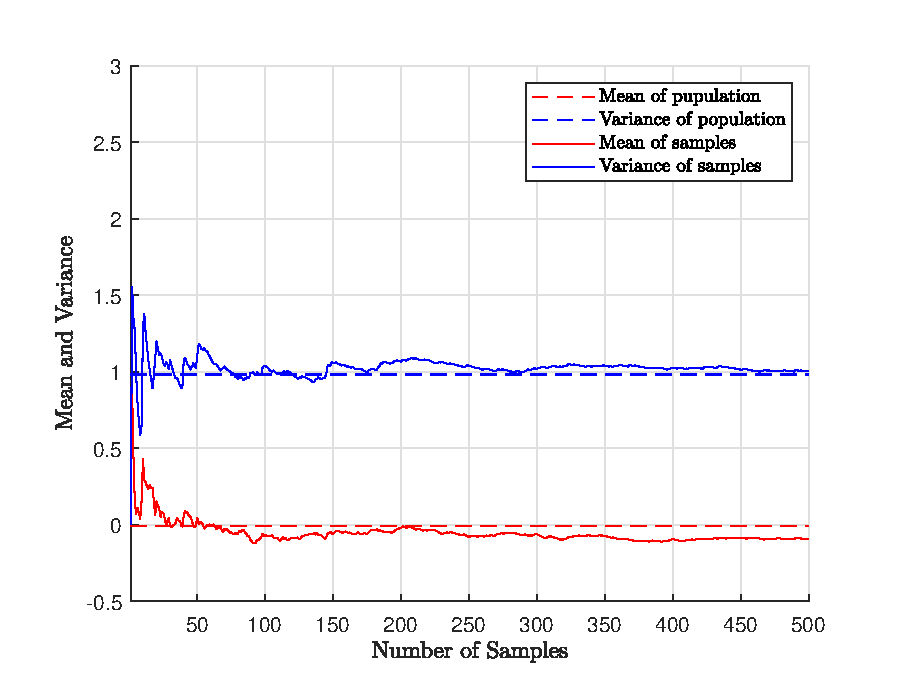
\includegraphics[width=250pt]{chapters/part-2/figures/sample-wr-n100.eps}
	\caption{Sample with replacement, population size $N=100$, sample size $0< M\leq500$.} \label{ch:sampling:fig:sample-wr-n100}
\end{figure}

\begin{figure}[!htb]
	\centering
	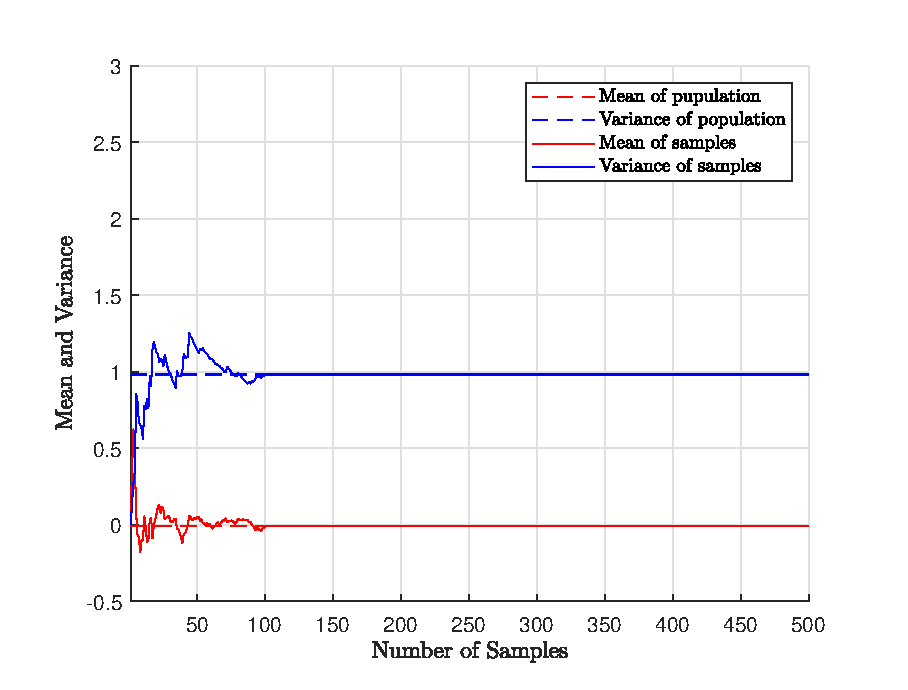
\includegraphics[width=250pt]{chapters/part-2/figures/sample-nwr-n100.eps}
	\caption{Sample without replacement, population size $N=100$, sample size $0< M\leq500$.} \label{ch:sampling:fig:sample-nwr-n100}
\end{figure}

In practice, however, the population size is often orders of magnitudes larger than the number of samples. In the second example, let $N=10000$ and $M=500$. The corresponding figures are given in Figs. \ref{ch:sampling:fig:sample-wr-n10000} and \ref{ch:sampling:fig:sample-nwr-n10000}. There is no obvious differences of the two figures.

\begin{figure}[!htb]
	\centering
	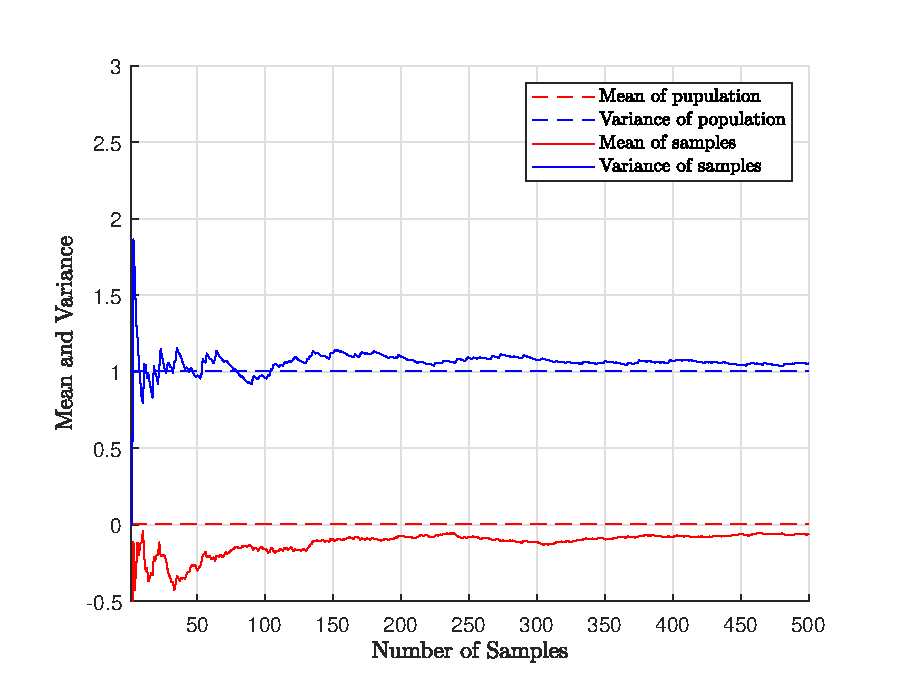
\includegraphics[width=250pt]{chapters/part-2/figures/sample-wr-n10000.eps}
	\caption{Sample with replacement, population size $N=10000$, sample size $0< M\leq500$.} \label{ch:sampling:fig:sample-wr-n10000}
\end{figure}

\begin{figure}[!htb]
	\centering
	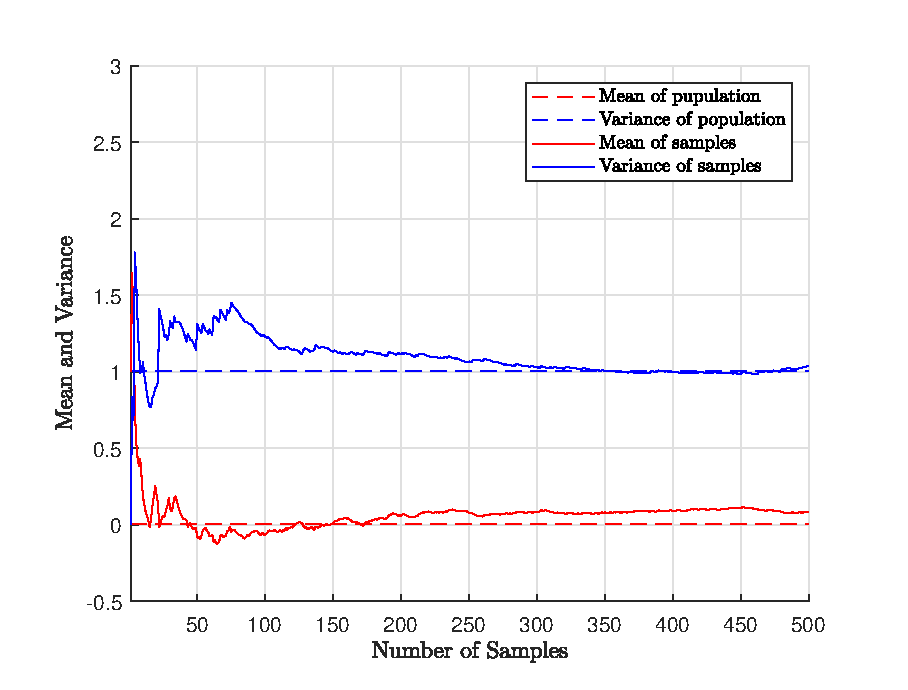
\includegraphics[width=250pt]{chapters/part-2/figures/sample-nwr-n10000.eps}
	\caption{Sample without replacement, population size $N=10000$, sample size $0< M\leq500$.} \label{ch:sampling:fig:sample-nwr-n10000}
\end{figure}

\section{Moments Estimation}

It is reasonable to assume that the statistical properties of the samples are connected with those of the population. The statistics of the population can be estimated using the samples. The larger the sample size, the more likely this statement holds true.

In practice, certain types of distributions of the population are often assumed based on prior knowledge or common sense, for example, Gaussian distribution for the salaries of people living in a city. Samples are taken from the population and used to estimate the properties of the distribution, such as its mean and variance.

More details are given below.

\subsection{Mean and Variance}

The \mync{sample mean} and \mync{sample variance} are calculated as follows. Let $X_1, \ldots, X_m$ be the samples. For sampling size $m\geq 2$,
\begin{eqnarray}
	\bar{X} &=& \dfrac{1}{m}\sum_{i=1}^{m}X_i \label{eq:sample_mean} \\
	S^2 &=& \dfrac{1}{m-1}\sum_{i=1}^{m}\left(X_i - \bar{X}\right)^2 \label{eq:sample_variance}
\end{eqnarray}

Do not confuse the sample mean in \eqref{eq:sample_mean} and sample variance in \eqref{eq:sample_variance} with the true population mean and variance, typically denoted by $\mu$ and $\sigma^2$. Although they are closely related, they are not the same.

According to LLN, the sample mean $\bar{X}$ converges to the population mean $\mu$ as the number of samples $m$ increases. It can be proved that the sample variance $S^2$ converges to the population variance $\sigma^2$ as well. The proof is given below.

From \eqref{eq:sample_variance},
\begin{eqnarray}
	E\left[S^2\right] &=& E\left[\dfrac{1}{m-1}\sum_{i=1}^{m}\left(X_i - \bar{X}\right)^2\right] \nonumber \\
	&=& \dfrac{1}{m-1} E\left[\sum_{i=1}^{m}\left(X_i^2 - 2X_i\bar{X} + \bar{X}^2\right)\right]  \nonumber \\
	&=& \dfrac{1}{m-1} E\left[\sum_{i=1}^{m}X_i^2 - 2\bar{X}\sum_{i=1}^{m}X_i + m\bar{X}^2\right] \label{eq:proof_samplevar_1} \\
	&=& \dfrac{1}{m-1} E\left[\sum_{i=1}^{m}X_i^2 - m\bar{X}^2\right] \nonumber \\
	&=& \dfrac{1}{m-1}\sum_{i=1}^{m} E\left[X_i^2\right] - \dfrac{m}{m-1}E\left[\left(\dfrac{1}{m}\sum_{i=1}^{m}X_i\right)^2\right] \nonumber \\
	&=& \dfrac{1}{m-1}\sum_{i=1}^{m} E\left[X_i^2\right] - \dfrac{1}{m(m-1)}E\left[\left(\sum_{i=1}^{m}X_i\right)^2\right] \label{eq:proof_samplevar_2} \\
	&=& \dfrac{1}{m-1}\sum_{i=1}^{m} \left(\textup{Var}(X_i) + E[X_i]^2\right) \nonumber \\ && -  \dfrac{1}{m(m-1)}\left(\textup{Var}\left(\sum_{i=1}^{m}X_i\right) + E\left[\sum_{i=1}^{m}X_i\right]^2\right) \nonumber \\
	&=& \dfrac{m}{m-1}\left(\sigma^2 + \mu^2\right) - \dfrac{1}{m(m-1)}\left(m\sigma^2 + m^2\mu^2\right) \nonumber \\
	&=& \dfrac{1}{m-1}\left(m\sigma^2 + m\mu^2 - \sigma^2 - m\mu^2\right) \nonumber \\
	&=& \sigma^2 \nonumber
\end{eqnarray}
where note that in \eqref{eq:proof_samplevar_1} 
\begin{eqnarray}
	\sum_{i=1}^{m}X_i &=& m\bar{X} \nonumber
\end{eqnarray}
which is from \eqref{eq:sample_mean}, and in \eqref{eq:proof_samplevar_2}
\begin{eqnarray}
	E\left[X^2\right] &=& \textup{Var}(X) + E[X]^2 \nonumber
\end{eqnarray}
for any random variable $X$ as given in \eqref{eq:varderived}.

The reason for dividing by $m-1$ in \eqref{eq:sample_variance}, rather than $m$, is that the sample mean $\bar{X}$ is also estimated from the data. This adjustment ensures that $S^2$ is an unbiased estimation of the population variance $\sigma^2$.

Imagine a scenario where the population mean $\mu$ is known in advance. In that case, we could have calculated sample variance alternatively as follows
\begin{eqnarray}
	{S^*}^2 &=& \dfrac{1}{m}\sum_{i=1}^{m}\left(X_i - \mu\right)^2 \nonumber
\end{eqnarray}
This estimator would also be unbiased for $\sigma^2$, and does not require the $m-1$ correction.

\subsection{Other Moments}

Recall from Section \ref{sec:moments} that the mean and the variance are the $1$st order moment and the $2$nd order central moment respectively. The mean and variance obtained from the samples are closely related their correspondents in the population. It is natural to expand the idea to other moments. This is known as the \mync{method of moments} in population estimation.

Commonly used moments and central moments are of $4$th order or lower. Note that bias might be introduced when using central moments where the center is obtained from the samples, as illustrated earlier for the sample variance.

\section{Confidence Interval Estimation}

The estimation obtained from empirical data often differs from the true value due to the randomness introduced by the samples. From CLT, we know that the more samples, the more confident we are that the true value is close to the estimate. 

To put it into perspective, we can derive the probability of the true value $\theta$ actually lying with a given interval $\left[\hat{\theta}_{\textup{min}},\hat{\theta}_{\textup{max}}\right]$, $P\left(\hat{\theta}_{\textup{min}} \leq \theta \leq \hat{\theta}_{\textup{max}}\right)$, as a function of estimation algorithm, measurement noise and samples number. The interval is known as the \mync{Confidence Interval}[CI]. Each CI corresponds with a probability. CI estimation tries to find the probability of a CI, or find the smallest CI for a given probability.

As an example, consider estimating the CI of the mean of a normal distribution using samples taken from that distribution. Let $\mathcal{N}(\mu,\sigma^2)$ be a normal distribution, and $X_1, \ldots, X_m$ a set of $m$ samples generated from the distribution. From the samples, the sample mean $\bar{X}$ and sample variance $S^2$ are calculated.

Apparently, $\mu$ does not necessarily equal to $\bar{X}$. The smaller $\sigma^2$ and larger $m$, the more likely that $\bar{X}$ is close to $\mu$. The error $\tilde{\mu} = \mu - \bar{X}$ is a random variable with
\begin{eqnarray}
	E[\tilde{\mu}] &=& 0 \nonumber \\
	\textup{Var}[\tilde{\mu}] &=& E\left[\left(\mu-\dfrac{1}{m}\sum_{i=1}^{m} X_i\right)^2\right] \nonumber \\
	&=& E\left[\left(\dfrac{1}{m}\sum_{i=1}^{m}\mu-\dfrac{1}{m}\sum_{i=1}^{m} X_i\right)^2\right] \nonumber \\
	&=& \dfrac{1}{m^2}E\left[\left(\sum_{i=1}^{m}\left(\mu-X_i\right)\right)^2\right] \label{eq:sample_mean_var0} \\
	&=& \dfrac{1}{m^2}E\left[\sum_{i=1}^{m}\left(\mu-X_i\right)^2\right] \label{eq:sample_mean_var1} \\
	&=& \dfrac{1}{m}\sigma^2 \label{eq:sample_mean_var2}
\end{eqnarray}
where notice that in \eqref{eq:sample_mean_var0},
\begin{eqnarray}
	E\left[\left(\mu-X_i\right)\left(\mu-X_j\right)\right] &=& 0 \nonumber
\end{eqnarray}
for $i\neq j$.

Though \eqref{eq:sample_mean_var2} can be used to derive the CI, it is useless in the empirical approach because the statistics of the original distribution, $\mu$ and $\sigma$, is not known exactly. Therefore, \eqref{eq:sample_mean_var2} needs to be reformulated to include $\bar{X}$ and $S^2$. Rewrite \eqref{eq:sample_mean_var1} as follows.
\begin{eqnarray}
	\textup{Var}[\tilde{\mu}] &=& \dfrac{1}{m^2}E\left[\sum_{i=1}^{m}\left(\bar{X}+\tilde{\mu}-X_i\right)^2\right] \nonumber \\
	&=& \dfrac{1}{m^2}E\left[\sum_{i=1}^{m}\left(\bar{X}-X_i\right)^2\right] + \dfrac{2}{m^2}E\left[\sum_{i=1}^{m}\left(\bar{X}-X_i\right)\tilde{\mu}\right] + \dfrac{1}{m^2}E\left[\sum_{i=1}^{m}\tilde{\mu}^2\right] \nonumber \\
	&=& \dfrac{m-1}{m^2}S^2 + \dfrac{1}{m}\textup{Var}[\tilde{\mu}] \label{eq:sample_mean_var3}
\end{eqnarray}
where notice that
\begin{eqnarray}
    E\left[\sum_{i=1}^{m}\left(\bar{X}-X_i\right)\tilde{\mu}\right] &=& 0 \nonumber
\end{eqnarray}

Solving \eqref{eq:sample_mean_var3} for $E[\tilde{\mu}^2]$ gives
\begin{eqnarray}
	\textup{Var}[\tilde{\mu}] &=& \dfrac{1}{m}S^2 \label{eq:sample_mean_var4}
\end{eqnarray}
Equations \eqref{eq:sample_mean_var2} and \eqref{eq:sample_mean_var4} look similar except that $\sigma^2$ is replaced by $S^2$. Notice that \eqref{eq:sample_mean_var4} gives the variance. For the standard deviation,
\begin{eqnarray}
	\textup{Std}(\tilde{\mu}) = \dfrac{1}{\sqrt{m}}\sqrt{S^2} = \dfrac{1}{\sqrt{m}}S \label{eq:sample_mean_var5}
\end{eqnarray} 
where $S$ is the estimate of the standard deviation using the samples. Let the interval be $\left[\bar{X}-\textup{CI}, \bar{X}+\textup{CI}\right]$ where from \eqref{eq:sample_mean_var5},
\begin{eqnarray}
	\textup{CI} &=& \dfrac{u_{\alpha}}{\sqrt{m}}S \label{eq:intervalci}
\end{eqnarray}
and $u_{\alpha}$ a gain factor determines the range of CI. Each $u_{\alpha}$ corresponds with a CI and a probability. The relation can be derived from the CDF. The result is given below.
\begin{eqnarray}
	\textup{F}(u_\alpha) = \dfrac{P+1}{2} = \dfrac{1}{2}\left(1+\textup{erf}\left(\dfrac{u_\alpha}{\sqrt{2}}\right)\right) \nonumber
\end{eqnarray}
where $F(\cdot)$ is the CDF of the standard normal distribution and $\textup{erf}(\cdot)$ the error function. This is equivalent with
\begin{eqnarray}
	\textup{erf}\left(\dfrac{u_\alpha}{\sqrt{2}}\right) &=& P \nonumber
\end{eqnarray}
Some commonly used $u_{\alpha}$ and confidence pairs are listed below for normal distribution noise assumption:
\begin{itemize}
	\item $u_{\alpha}=1$, $P=0.683$;
	\item $u_{\alpha}=1.96$, $P=0.95$;
	\item $u_{\alpha}=2$, $P=0.954$;
	\item $u_{\alpha}=2.58$, $P=0.99$;
	\item $u_{\alpha}=3$, $P=0.997$;
	\item $u_{\alpha}=3.29$, $P=0.999$.
\end{itemize}

In the previous example, the problem is to estimate the CI of the mean of a normal distribution. In practice, there are many other problems. 

For example, instead of using normal distribution as the noise assumption, $t$-distribution might be used, especially if the number of samples are small. The $t$-distribution has the ``heavy tail'' to emulate outliers, thus making the result more robust.

Depending on the choice of noise assumption, CI may look different and/or $u_{\alpha}$ may differ. There are CI tables for different types of noise.

